% Preamble:
% \usepackage{tikz}
% \usepackage{xcolor}

\begin{figure}[ht]
\centering
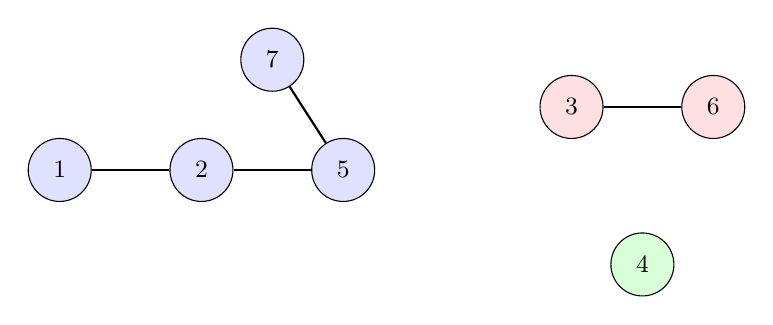
\begin{tikzpicture}[
  v/.style={circle, draw, minimum size=8mm, font=\small},
  blueV/.style={v, fill=blue!12},
  redV/.style={v, fill=red!12},
  greenV/.style={v, fill=green!15},
  e/.style={thick}
]

% --- Component C1 = {1,2,5,7} (blue) ---
\node[blueV] (1) at (0,0)   {1};
\node[blueV] (2) at (1.8,0) {2};
\node[blueV] (5) at (3.6,0) {5};
\node[blueV] (7) at (2.7,1.4) {7};

\draw[e] (1)--(2);
\draw[e] (2)--(5);
\draw[e] (5)--(7);

% --- Component C2 = {3,6} (red) ---
\node[redV] (3) at (6.5,0.8) {3};
\node[redV] (6) at (8.3,0.8) {6};
\draw[e] (3)--(6);

% --- Component C3 = {4} (green, isolated) ---
\node[greenV] (4) at (7.4,-1.2) {4};

\end{tikzpicture}
\caption{A disconnected graph with three connected components:
\textcolor{blue}{$\{1,2,5,7\}$}, \textcolor{red}{$\{3,6\}$}, and \textcolor{green}{$\{4\}$}.
The subgraph on $\{3,4,6\}$ is not connected because vertex $4$ is isolated from $\{3,6\}$, while the subgraph on $\{1,2,5\}$ is not maximal since it can be enlarged to the connected component $\{1,2,5,7\}$.}
\label{fig:components-example}
\end{figure}
